\section{Descrição do Problema}

Imagine dividir uma turma em dois times. Cada par de pessoas tem um número, o \emph{peso}: positivo se queremos separar os dois (rivalidade), negativo se preferimos que fiquem juntos. O objetivo é escolher os times de modo que a soma dos pesos dos pares \emph{separados} seja a maior possível.

Formalmente, temos um grafo não direcionado $G=(V,E)$ com $n$ vértices e $m$ arestas, e cada aresta $uv$ tem um peso inteiro $w_{uv}$. Uma partição atribui a cada vértice o lado 0 ou 1, e o valor do corte é a soma dos pesos das arestas cujas pontas ficam em lados diferentes. Queremos a partição de maior valor, $\mathrm{OPT}$. A notação é a mesma do Trabalho~1: $N(v)$ é a vizinhança de $v$ e $\Delta$ é o grau máximo.

\subsection{Complexidade}

O problema é NP-difícil \cite{Karp 1972, Garey et al. 1976}: não se conhece, e não se espera, um algoritmo que seja rápido em todos os casos. A forma mais direta de resolvê-lo é testar todas as divisões possíveis, $2^{n-1}$ delas (com $n=100$ são cerca de $10^{30}$, inviável). O melhor limite teórico conhecido para o caso geral é de ordem $1{,}73^n$ \cite{Williams 2005}, que ainda é exponencial e usa muita memória. Na prática, o que ajuda é a \emph{estrutura} do grafo: em grafos planares o problema tem solução rápida \cite{Hadlock 1975}, e em grafos que podem ser ``varridos'' com uma frente de largura $w$ ele se resolve em tempo proporcional a $2^{w}$ \cite{Arnborg et al. 1991, Bodlaender 1993}, o que é rápido se $w$ for pequeno. Esse é o caso das nossas grades toroidais estreitas, e é a ideia do segundo algoritmo.

\section{Estado da Arte em Algoritmos Exatos}

Os métodos exatos usados na prática para o Max-Cut se dividem em três famílias.

\paragraph{Branch-and-cut (programação linear).} Transforma o problema em um problema de programação linear e vai acrescentando restrições (desigualdades) que cortam soluções impossíveis. Foi aplicado a estados fundamentais de vidros de spin e ao projeto de circuitos \cite{Barahona et al. 1988}, e \citet{Liers et al. 2004} descrevem seu uso em casos difíceis. \citet{Liers et al. 2003} resolveram grafos aleatórios regulares de grau 4 e 6 com até 1\,280 vértices, classe parecida com os nossos aleatórios esparsos (que têm grau médio 4). É, em geral, o método mais indicado para grafos esparsos.

\paragraph{Branch-and-bound semidefinido.} Usa uma relaxação mais forte (programação semidefinida) para calcular os limites. O \emph{Biq Mac} \cite{Rendl et al. 2010} resolve qualquer instância com até 100 vértices, qualquer que seja a densidade, e é a referência para grafos densos; os autores observam que, para grafos esparsos, os métodos de programação linear podem ser melhores. \citet{Krislock et al. 2014} melhoraram o cálculo desses limites.

\paragraph{Aproveitar a estrutura do grafo.} Para grafos de largura de caminho ou de árvore pequena, a programação dinâmica é exata e custa $O(2^{w}\cdot\mathrm{poly}(n))$ \cite{Arnborg et al. 1991, Bodlaender 1993}. A largura de caminho é a menor ``frente de varredura'' que se consegue em alguma ordem dos vértices \cite{Kinnersley 1992}, o que permite implementar a ideia como um simples percurso, como fazemos na Seção~5.2.

Nossos algoritmos são versões simples dessas ideias: o Branch-and-Bound usa um limite bem mais barato (e mais fraco) que os das duas primeiras famílias, e a programação dinâmica é a versão mais básica da terceira. Não esperamos competir com o \emph{Biq Mac} nem com os resolvedores de branch-and-cut, e a comparação da Seção~7 deve ser lida com esse cuidado.

\section{Técnicas Escolhidas}

\paragraph{Branch-and-Bound: tentar e podar.} É como percorrer um labirinto de decisões. Escolhemos o lado de um vértice de cada vez (duas opções), formando uma árvore de possibilidades. Antes de seguir por um ramo, calculamos um \emph{teto}: o melhor corte que ainda seria possível nesse ramo, na melhor das hipóteses. Se o teto não supera a melhor solução já encontrada, o ramo inteiro é descartado (podado), sem precisar visitá-lo. Quanto mais justo o teto, mais se poda. Começamos com a heurística do Trabalho~1 como ``melhor solução já vista'', o que liga os dois trabalhos: uma heurística boa poda mais desde o início.

\paragraph{Programação dinâmica: lembrar só o necessário.} É como ler um livro de capítulo em capítulo anotando num quadro só o que ainda será citado adiante. Processamos os vértices em uma ordem fixa. O \emph{quadro} é a \emph{fronteira}: os vértices já processados que ainda têm vizinhos por processar. Para cada combinação de lados dos vértices do quadro, guardamos o melhor valor obtido até ali. Quando um vértice perde o último vizinho pendente, ele sai do quadro, e ficamos com o melhor de seus dois lados. A Figura~\ref{fig:fronteira} mostra o percurso. O custo cresce com o tamanho do quadro (a largura $w$), e não com $n$.

As duas técnicas se complementam. O Branch-and-Bound funciona em qualquer grafo, mas o tempo explode com $n$ mesmo em grafos esparsos. A programação dinâmica depende de o grafo ter uma frente de varredura pequena, mas, quando tem, resolve instâncias com dezenas de milhares de vértices.

\begin{figure}[ht]
\centering
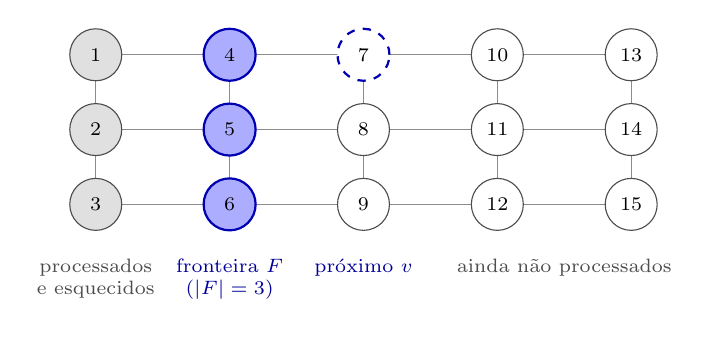
\begin{tikzpicture}[x=1.7cm,y=-0.95cm,
  vtx/.style={circle,draw=black!70,minimum size=0.66cm,inner sep=0pt,font=\scriptsize},
  proc/.style={vtx,fill=black!12},
  fron/.style={vtx,fill=blue!32,draw=blue!70!black,thick},
  prox/.style={vtx,fill=white,draw=blue!70!black,thick,dashed},
  nao/.style={vtx,fill=white},
  aresta/.style={draw=black!45}]
  \foreach \c in {1,...,5}{\foreach \r in {1,2,3}{
    \pgfmathtruncatemacro{\id}{(\c-1)*3+\r}
    \coordinate (p\c\r) at (\c,\r);
  }}
  \foreach \c in {1,...,5}{\foreach \r in {1,2,3}{
    \pgfmathtruncatemacro{\cc}{\c+1}\pgfmathtruncatemacro{\rr}{\r+1}
    \ifnum\c<5 \draw[aresta] (p\c\r) -- (p\cc\r); \fi
    \ifnum\r<3 \draw[aresta] (p\c\r) -- (p\c\rr); \fi
  }}
  \foreach \c/\sty in {1/proc,2/fron,3/nao,4/nao,5/nao}{\foreach \r in {1,2,3}{
    \pgfmathtruncatemacro{\id}{(\c-1)*3+\r}
    \ifnum\c=3\ifnum\r=1 \node[prox] at (p\c\r) {\id}; \else \node[nao] at (p\c\r) {\id}; \fi
    \else \node[\sty] at (p\c\r) {\id}; \fi
  }}
  \node[anchor=north,align=center,font=\scriptsize,text=black!70] at (1,3.6) {processados\\e esquecidos};
  \node[anchor=north,align=center,font=\scriptsize,text=blue!60!black] at (2,3.6) {fronteira $F$\\($|F|=3$)};
  \node[anchor=north,align=center,font=\scriptsize,text=blue!60!black] at (3,3.6) {próximo $v$};
  \node[anchor=north,align=center,font=\scriptsize,text=black!70] at (4.5,3.6) {ainda não processados};
\end{tikzpicture}
\caption{Percurso da programação dinâmica em uma grade $3\times5$ numerada por colunas. Os vértices 1 a 3 já saíram da fronteira (todos os seus vizinhos foram processados); os vértices 4 a 6 formam a fronteira $F$, porque cada um ainda tem vizinho na coluna seguinte. Ao inserir o vértice 7, a tabela tem $2^{|F|+1}=16$ entradas.}\label{fig:fronteira}
\end{figure}

